\documentclass[a0paper,portrait,fontscale=0.34]{baposter}

\usepackage{relsize}		% For \smaller
\usepackage{epstopdf}	  % Included EPS files automatically converted to PDF to include with pdflatex
\usepackage{url}			  % For \url
\usepackage{multicol}
\usepackage{amsmath}
\usepackage{empheq}
\usepackage{graphicx} % Required for including images
\usepackage{hyperref}
% \NeedsTeXFormat{LaTeX2e}
% \ProvidesPackage{ThesisCommands}[2016/06/20 ThesisCommands]

\usepackage{amsmath}
\usepackage{amsfonts}
\usepackage{calc}
% \DeclareMathOperator{\sgn}{sgn}
% \newcommand{\expnumber}[2]{{#1}\mathrm{e}{#2}}
%%%%%%%%%%%%%%%%%%%%%%%%%%%%%%%%%%%%%%%%%%%%%%%%%%%%%%%% General %%%%%%%%%%%%%%%%%%%%%%%%%%%%%%%%%%%%%%%%%%%%%%%%%%%%%%%%
%Font
\newcommand{\bm}[1]{\text{\boldmath $#1$\unboldmath}}
\newcommand{\bb}{\mathbf}
\newcommand{\cc}{\mathcal}
\newcommand{\ang}{\mbox{\normalfont\AA}}
% Operators
\newcommand{\dP}{\partial}
\newcommand{\dPx}[1]{\frac{\dP #1}{\dP x_1}}
\newcommand{\dPy}[1]{\frac{\dP #1}{\dP x_2}}
\newcommand{\dPz}[1]{\frac{\dP #1}{\dP x_3}}
\newcommand{\Dxk}[1]{\frac{\dP #1}{\dP x_k}}
\newcommand{\dPk}[2]{\frac{\dP #2}{\dP #1 }}
\newcommand{\Dt}[1]{\frac{\dP  #1}{\dP t  }}
\newcommand{\dt}[1]{\frac{d    #1}{dt     }}
\newcommand{\dx}[1]{\frac{d    #1}{dx     }}
\newcommand{\dxTwo}[1]{\frac{d^2 #1}{dx^2   }}
\newcommand{\dxk}[2]{\frac{d   #1}{d#2    }}
\newcommand{\grad}{\bm{\nabla}}
\renewcommand{\div}{\bm{\nabla}\cdot}
\newcommand{\rot}{\bm{\nabla}\times}
\newcommand{\jump}[1]{\llbracket {#1} \rrbracket}
% Sum,Int
\newcommand{\IntE}{\int_{\Omega_{e}}}
\newcommand{\IntG}{\int_{\partial\Omega_{e}}}
\newcommand{\Intg}{\int_{\Gamma}}
\newcommand{\dG}{d\Gamma}
\newcommand{\sumD}[1]{\underset{#1}{\sum}}
\newcommand{\sumUD}[2]{\overset{#1}{\underset{#2}{\sum}}}
\newcommand{\sumDU}[2]{\overset{#2}{\underset{#1}{\sum}}}
\newcommand{\intInfty}{\int_{0}^{+\infty} }
\newcommand{\intInf}{\int_{-\infty}^{+\infty} }
\newcommand{\intV}{\int\int\int_V}
\newcommand{\intS}{\int\int_S}
\newcommand{\sumInf}{\overset{+\infty}{\underset{-\infty}{\sum}}}
\newcommand{\limInf}[1]{\underset{#1 \rightarrow\infty}{\rightarrow}}
\newcommand{\Lim}[2]{\underset{#1 \rightarrow {#2}}{lim}}


%%%%%%%%%%%%%%%%%%%%%%%%%%%%%%%%%%%%%%%%%%%%%%%%%% Quantum mechnaics %%%%%%%%%%%%%%%%%%%%%%%%%%%%%%%%%%%%%%%%%%%%%%%%%%%%%%%%%%%%%
\newcommand{\braket}[1]{\langle #1 \rangle}
\newcommand{\bra}[1]{\langle #1 }
\newcommand{\ket}[1]{#1 \rangle}
\newcommand{\matrixElem}[3]{\left\langle #1 | #2 | #3 \right\rangle}
\newcommand{\matElem}[3]{\matrixElem{#1}{#2}{#3}}
\newcommand{\Mm}{\begin{array}{c}max\\min \end{array}}
\newcommand{\hbm}{\frac{\hbar}{m_0}}
\newcommand{\hbsm}{\frac{\hbar^2}{2m_0}}
\newcommand{\hbsme}[1]{\frac{\hbar^2}{2m_{#1} }}
\newcommand{\hbksm}{\frac{\hbar^2k^2}{2m_0 } }
\newcommand{\hbksme}[1]{\frac{\hbar^2k^2}{2m_{#1} }}
\newcommand{\smhb}[1]{\frac{2m_0 #1}{\hbar^2}}
\newcommand{\Vqdim}{\tilde V_0}


%Hydrogen
\newcommand{\emphi}[1]{e^{#1 j\varphi}}
\newcommand{\cmp}[1]{ \cos#1\varphi}
\newcommand{\smp}[1]{ \sin#1\varphi}
\newcommand{\cmt}[1]{ \cos^{#1}\theta}
\newcommand{\smt}[1]{ \sin^{#1}\theta}
\newcommand{\cp}{ \cos\varphi}
\renewcommand{\sp}{ \sin\varphi}
\newcommand{\ct}{ \cos\theta}
\newcommand{\st}{ \sin\theta}
\newcommand{\sqfopi}{\frac{1}{\sqrt{4\pi}}}
\newcommand{\sqf}[2]{\sqrt{\frac{#1}{#2}}}

%kp Theory
\newcommand{\Psik}{\Psi_{\bb k}(\bb r)}
\newcommand{\PsiO}{\Psi^{(0)}}
\newcommand{\EnO}{\E^{(0)}_n}
\newcommand{\ukr}{u_{\bb k}(\bb r)}
\newcommand{\unkr}{u_{n,\bb k}(\bb r)}%^{(n)}
\newcommand{\unk}{u_{n,\bb k}}
\newcommand{\Enk}{E_{n,\bb k}}
\newcommand{\kdotr}{\bb k\cdot\bb r}
\newcommand{\kdotp}{\bb k\cdot\bb p}
\newcommand{\conj}{\dagger}
\newcommand{\tildeR}{\tilde R}
\newcommand{\tildeRconj}{\tilde R^{\conj}}

% Quantum well
\newcommand{\kzQ}{k_z}
\newcommand{\kza}{k}
\newcommand{\kt}{k_t}
\newcommand{\kzb}{\kappa}
\newcommand{\wdt}{w}
\newcommand{\adt}{a}
\newcommand{\me}{m_e}
\newcommand{\mea}{m_w}
\newcommand{\meb}{m_b}
\newcommand{\mz}{m_z}
\newcommand{\mt}{m_t}
\newcommand{\mza}{m_{z,w}}
\newcommand{\mzb}{m_{z,b}}
\newcommand{\mta}{m_{t,w}}
\newcommand{\mtb}{m_{t,b}}
\newcommand{\pj}{p_{j,j+1}}
\newcommand{\kzl}{k_{(j+1)z}l_{j+1}}
\newcommand{\kzi}{k_{i,z}}
\newcommand{\krho}{k_{\rho}}
\newcommand{\krhoDim}{\tilde{\krho}}
%\newcommand{\kz}{k_{z}}
%kzj
\newcommand{\kzHLj}[1]{ k_{#1,z}^{(j)} }
\newcommand{\kzHHj}{\kzHLj{HH}}
\newcommand{\kzLHj}{\kzHLj{LH}}
%A,B
\newcommand{\ABLHj}[2]{#1_{#2}^{(j)}}
\newcommand{\AHHj}{\ABLHj{A}{HH}}
\newcommand{\ALHj}{\ABLHj{A}{LH}}
\newcommand{\BHHj}{\ABLHj{B}{HH}}
\newcommand{\BLHj}{\ABLHj{B}{LH}}
%F
\newcommand{\FHp}[2]{ \bb F_{#1}^{(j#2)}  }
\newcommand{\FHHjp}{\FHp{HH}{+}}
\newcommand{\FLHjp}{\FHp{LH}{+}}
\newcommand{\FHHjm}{\FHp{HH}{-}}
\newcommand{\FLHjm}{\FHp{LH}{-}}

\newcommand{\mei}{m_{i}}
\newcommand{\Rt}{\tilde R}
\newcommand{\Rtd}{\Rt^{\dagger}}
%
\newcommand{\vecHorz}[1]{\left(#1 \right)}
\newcommand{\vecTwo}[2]{\left[\begin{array}{c} #1 \\ #2 \end{array}\right]}
\newcommand{\diagTwo}[2]{\left[\begin{array}{cc} #1 & 0 \\ 0 & #2 \end{array}\right]}
\newcommand{\matTwo}[4]{\left[\begin{array}{cc} #1 & #2 \\ #3 & #4 \end{array}\right]}
\newcommand{\matFour}[4]{\left[\begin{array}{cccc} #1\\ #2\\ #3\\ #4 \end{array}\right]}
\newcommand{\mBar}{\bar m}
\newcommand{\cBar}{\bar c}

%%%%% Gain
\renewcommand{\k}{\bb k}
\newcommand{\kpar}{\bb k_{||}}
\newcommand{\Epar}{E_{||}}
\newcommand{\rhoif}{\rho(\omega_{fi})}
\newcommand{\eikr}{e^{j\k\cdot\bb r}}
\newcommand{\Evar}{\varepsilon}
\newcommand{\mrme}{\frac{m_r}{m_e}}
\newcommand{\mrmh}{\frac{m_r}{m_h}}

%\newcommand{\Eint}{\varepsilon}



%%%%%%%%%%%%%%%%%%%%%%%%%%%%%%%%%%%%%%%%%%%%%%%%%%%%%%%%%%%%%%%%%%%%%%%%%%%%%%%%%%%%%%%%%%%%%%%%%%%%%%%%%%%%%%%%%%%%%%%%%%%%%%%%%%%%%%
%%%%%%%%%%%%%%%%%%%%%%%%%%%%%%%%%%%%%%%%%%%%%%%%%%%%%%%% Electrical modelling %%%%%%%%%%%%%%%%%%%%%%%%%%%%%%%%%%%%%%%%%%%%%%%%%%%%%%%%
% Poisson solver Dim constants
\newcommand{\varphiDim}{\tilde\varphi}
\newcommand{\phiDim}{\tilde\phi}
\newcommand{\Vdim}{\tilde V}
\newcommand{\Kf}{\bb K^{\ast}}
% Rate eq
\newcommand{\pvDim}{\tilde{p}_v}
\newcommand{\ncDim}{\tilde{n}_c}
\newcommand{\JnDim}{\tilde{\bm J}_n}
\newcommand{\JpDim}{\tilde{\bm J}_p}
\newcommand{\UnDim}{\tilde{U}_n}
\newcommand{\UpDim}{\tilde{U}_p}
\newcommand{\GnDim}{\tilde{G}_n}
\newcommand{\GpDim}{\tilde{G}_p}
\newcommand{\VnDim}{\tilde{\phi}_n}
\newcommand{\VpDim}{\tilde{\phi}_p}
\newcommand{\td}{d}
% SemiConductor statistics Dim Constants
\newcommand{\PsiDim}{\tilde\Psi}
\newcommand{\FnDim}{\tilde{F}_n}
\newcommand{\FpDim}{\tilde{F}_p}
\newcommand{\DnDim}{\tilde{D}_n}
\newcommand{\DpDim}{\tilde{D}_p}
\newcommand{\Ek}{\varepsilon}
\newcommand{\EFp}{E_{F,p}}
\newcommand{\EFn}{E_{F,n}}

% Rate eq weak formulation
\newcommand{\Jdrift }{\bb J^{drift}}
\newcommand{\Jdiff  }{\bb J^{diff}}
\newcommand{\dJdrift}{\bb dJ^{drift}}
\newcommand{\dJdiff }{\bb dJ^{diff}}
\newcommand{\dJdriftP}{\dPk{\phi_{p,k}}{\Jdrift}}
\newcommand{\dJdiffP }{\dPk{\phi_{p,k}}{\Jdiff }}
\newcommand{\dJdriftN}{\dPk{\phi_{n,k}}{\Jdrift}}
\newcommand{\dJdiffN }{\dPk{\phi_{n,k}}{\Jdiff }}
\newcommand{\dUp}{\dPk{\phi_{p,k}}{\bb U} }
\newcommand{\dUn}{\dPk{\phi_{n,k}}{\bb U} }

%Lateral rate eq perturb
\newcommand{\pv}{p_v(x)}
\newcommand{\nc}{n_c}
\newcommand{\Gmod}{G}
\newcommand{\Uss}{\bar\gamma_s}%U_{ss}}
\newcommand{\gN}{\bar g_0}
\newcommand{\gs}{\bar g_0}
\newcommand{\Ux}{U(x)}
\newcommand{\Iem}{\cc I_m}
\newcommand{\betaN}{\bar\beta}
\newcommand{\Ginj}{G_{inj}}
\newcommand{\Rsp}{R_{sp}}
\newcommand{\Veff}{V_{eff}}
\newcommand{\Va}{V_{a}}
\renewcommand{\SS}[1]{\bar #1}
\newcommand{\SSpv}{\bar{p}_v(x)}
\newcommand{\Sss}{S}
\newcommand{\Nss}{N}
\newcommand{\Iinj}{I}%\frac{\eta I}{qV_a}}
\newcommand{\Ldeff}{L_{D,eff}}


%%%%%%%%%%%%%%%%%%%%%%%%%%%%%%%%%%%%%%%%%%%%%% Optical Modelling  Electromagnetism %%%%%%%%%%%%%%%%%%%%%%%%%%%%%%%%%%
%constant
\newcommand{\oneHalf}{\frac{1}{2}}
\newcommand{\eps}{\epsilon}
\newcommand{\oneEps}{\frac{1}{\eps}}
\newcommand{\oneMu}{\frac{1}{\mu}}
\newcommand{\oneEta}{\frac{1}{\eta}}
\newcommand{\epsInf}{\epsilon_{\infty}}
\newcommand{\epsI}{\eps''}
\newcommand{\epsR}{\eps'}
%Vectors
% \renewcommand{\r}{\bm{r}}
\newcommand{\E}{\bm{E}}
\renewcommand{\H}{\bm{H}}
\newcommand{\B}{\bm{B}}
\newcommand{\D}{\bm{D}}
\newcommand{\J}{\bm{J}}
\newcommand{\M}{\bm{M}}
\newcommand{\A}{\bm{A}}
\newcommand{\F}{\bm{F}}
\newcommand{\N}{\bm{N}}
\renewcommand{\L}{\bm{L}}
%
\renewcommand{\P}{\bm{P}}
\newcommand{\U}{\bm{U}}
\newcommand{\n}{\bm{n}}

%%%% Electromagnetism Dim
%constant
\newcommand{\xkDim}{\tilde{x_k}}
\newcommand{\tDim}{\tilde{t}}
\newcommand{\epsDim}{\tilde{\eps}}
\newcommand{\muDim}{\tilde{\mu}}
\newcommand{\sigmaDim}{\tilde{\sigma}}
\newcommand{\omegaDim}{\tilde{\omega}}
\newcommand{\gammaDim}{\tilde{\gamma}}
\newcommand{\etaDim}{\tilde{\eta}}
%Vectors
\newcommand{\Edim}{\tilde{\bm{E}}}
\newcommand{\Hdim}{\tilde{\bm{H}}}
\newcommand{\Bdim}{\tilde{\bm{B}}}
\newcommand{\Ddim}{\tilde{\bm{D}}}
\newcommand{\Jdim}{\tilde{\bm{J}}}
\newcommand{\Pdim}{\tilde{\bm{P}}}
\newcommand{\Mdim}{\tilde{\bm{M}}}
\newcommand{\Adim}{\tilde{\bm{A}}}
\newcommand{\Udim}{\tilde{\bm{U}}}
\newcommand{\xdim}{\tilde{\bm{x}}}
%Operators
\newcommand{\DtDim}[1]{\frac{\partial #1}{\partial\tDim}}
\newcommand{\nablaDim}{\tilde{\bm{\nabla}}}
\newcommand{\gradDim}{\bm{\nablaDim}}
\newcommand{\divDim}{\nablaDim\cdot}



%%%%%%%%%%%%%%%%%%%%%%%%%%%%%%%%%%%%%%%%%%%%%%%%%%%% misc
\newcommand{\spherProp}{\frac{e^{-j\beta r}}{r} }

%%% Electromagnetism Components
\newcommand{\Ex}{E_1}
\newcommand{\Ey}{E_2}
\newcommand{\Ez}{E_3}
\newcommand{\Hx}{H_1}
\newcommand{\Hy}{H_2}
\newcommand{\Hz}{H_3}
\newcommand{\Dx}[1]{\frac{\partial #1}{\partial x}}
\newcommand{\Dy}[1]{\frac{\partial #1}{\partial y}}
\newcommand{\Dz}[1]{\frac{\partial #1}{\partial z}}
\newcommand{\ex}{\bb e_x}
\newcommand{\ey}{\bb e_y}
\newcommand{\ez}{\bb e_z}
\newcommand{\kx}{k_x}
\newcommand{\ky}{k_y}
\newcommand{\kz}{k_z}
\newcommand{\ku}{k_{\bm u}}
\newcommand{\Ee}{\cc E_e}
\newcommand{\Em}{\cc E_m}
\newcommand{\Eem}{\cc E_{em}}


%%%%%%%%%%%%%%%%%%%%%%%%%%%%%%%%%%%%%%%% DGTD
\newcommand{\sumK}{\sumUD{nsd}{k=1}}
\newcommand{\FF}{\mathbb{F}}
%\newcommand{\F}{\bm{F}}
\newcommand{\Fk}{\F_k}
\newcommand{\Fx}{\F_1}
\newcommand{\Fy}{\F_2}
\newcommand{\Fz}{\F_3}
\newcommand{\Fn}{\bm{F}_{\n}}
\newcommand{\FNum}{\tilde{\F}_{\n}}
\renewcommand{\S}{\bm{S}}
\newcommand{\W}{\bm{W}}
%\newcommand{\A}{\bm{A}}
\newcommand{\An}{\A_{\n}}
\newcommand{\AnM}{\An^-}
%Discrete DGTD
\newcommand{\iN}{i\in\llbracket 1,N\rrbracket}
\newcommand{\jN}{j\in\llbracket 1,N\rrbracket}
\newcommand{\Li}{L_i}
\newcommand{\Lj}{L_j}
\newcommand{\Lk}{L_k}
\newcommand{\MijE}{M_{ij}^{\Omega_e}}
\newcommand{\Cijk}{C_{ij,k}^{\Omega_e}}
\newcommand{\MijG}{\bb M_{ij}^{\Gamma}}
\newcommand{\FDG}{\cc F^{DG}}
\newcommand{\Am}{\bb A^-_{\bb n}}
\newcommand{\Uxt}{\bar{\bb U}}
%Elt
\newcommand{\Uelt}{ \bb U^e}
\newcommand{\Melt}{ \bb M^{\Omega_e}}
\newcommand{\CxElt}{\bb C_1^{\Omega_e}}
\newcommand{\CyElt}{\bb C_2^{\Omega_e}}
\newcommand{\MgElt}{\bb M^{\gamma_e}}


%%%%%%%%%%%%%%%%%%%%%%%%%%%%%%%%%%%%%%%%%%%%%%%% Scattering
\newcommand{\RCS}{\sigma_{3D}}



%%%%%%%%%%%%%%%%%%%%%%%%%%%%%%%%%%%%%%%%%%%%%%%% Maths
%%%%%% Cyl/spherical coordinates
\newcommand{\sinc}{sinc}



%%%%%% Cyl/spherical coordinates
\newcommand{\er}{\bb e_r}
\newcommand{\etheta}{\bb e_{\theta}}
\newcommand{\ephi}{\bb e_{\phi}}
%
\newcommand{\Er}{E_r}
\newcommand{\Et}{E_{\phi}}
\newcommand{\Hr}{H_r}
\newcommand{\Ht}{H_{\phi}}
%
\newcommand{\dPr}{\dP_r}
\newcommand{\dPp}{\frac{1}{r}\dP_{\phi}}
\newcommand{\dPrho}{\dP_{\rho}}
\newcommand{\dPtheta}{\dP_{\theta}}
\newcommand{\dPphi}{\dP_{\phi}}
%
\newcommand{\Utheta}{U_{\theta}}
\newcommand{\Uphi}{U_{\phi}}
\newcommand{\Urho}{U_{\rho}}
\newcommand{\Uphip}{U_{\phi'}}

\newcommand{\Ltheta}{L_{\theta}}
\newcommand{\Lphi}{L_{\phi}}
\newcommand{\Ntheta}{N_{\theta}}
\newcommand{\Nphi}{N_{\phi}}
%
\newcommand{\ctheta}{\cos\theta}
\newcommand{\stheta}{\sin\theta}
\newcommand{\cphi}{\cos\phi}
\newcommand{\sphi}{\sin\phi}
%
\newcommand{\Jm}{J_m}
\newcommand{\Nm}{I_m}
\newcommand{\Km}{K_m}
\newcommand{\Ym}{Y_m}
%
\newcommand{\vecThree}[3]{\left[\begin{array}{c} #1 \\ #2 \\ #3 \end{array}\right]}
\newcommand{\matThree}[9]{\left[\begin{array}{ccc} #1 & #2 & #3 \\ #4 & #5 & #6 \\ #7 & #8 & #9 \end{array}\right]}

\newcommand\widecolourbox[1]{{\setlength\fboxrule{1.5pt}\setlength\fboxsep{11pt}\fcolorbox{red}{eqcolor}{\enspace#1\enspace }}}

\newcommand{\highlight}[1]{\textbf{\color{goodcol}#1\color{fscol}}}
\newcommand{\negCol}[1]{\textbf{\color{badcol}#1\color{fscol}}}

%%% Global Settings %%%%%%%%%%%%%%%%%%%%%%%%%%%%%%%%%%%%%%%%%%%%%%%%%%%%%%%%%%%
\graphicspath{{fig/}}	% Root directory of the pictures
\tracingstats=2			% Enabled LaTeX logging with conditionals


%%% Color Definitions %%%%%%%%%%%%%%%%%%%%%%%%%%%%%%%%%%%%%%%%%%%%%%%%%%%%%%%%%
\definecolor{goodcol}{RGB}{0,150,0}
\definecolor{badcol}{RGB}{150,0,0}
\definecolor{fscol}{RGB}{0,0,0}
% \definecolor{bgcol}{RGB}{150,200,230}
\definecolor{bgcol}{RGB}{200,230,250}
\definecolor{bordercol}{RGB}{23,55,94}
\definecolor{headercol1}{RGB}{23,55,94}
\definecolor{headercol2}{RGB}{65,95,150}
\definecolor{headerfontcol}{RGB}{255,255,255}
\definecolor{eqcolor}{RGB}{200,230,250}
% \definecolor{boxcolor}{RGB}{160,210,235}
\definecolor{boxcolor}{RGB}{220,240,255}

%%%%%%%%%%%%%%%%%%%%%%%%%%%%%%%%%%%%%%%%%%%%%%%%%%%%%%%%%%%%%%%%%%%%%%%%%%%%%%%%
%%% Utility functions %%%%%%%%%%%%%%%%%%%%%%%%%%%%%%%%%%%%%%%%%%%%%%%%%%%%%%%%%%

%%% Save space in lists. Use this after the opening of the list %%%%%%%%%%%%%%%%
\newcommand{\compresslist}{
	\setlength{\itemsep}{1pt}
	\setlength{\parskip}{0pt}
	\setlength{\parsep}{0pt}
}

%%%%%%%%%%%%%%%%%%%%%%%%%%%%%%%%%%%%%%%%%%%%%%%%%%%%%%%%%%%%%%%%%%%%%%%%%%%%%%%
%%% Document Start %%%%%%%%%%%%%%%%%%%%%%%%%%%%%%%%%%%%%%%%%%%%%%%%%%%%%%%%%%%%
%%%%%%%%%%%%%%%%%%%%%%%%%%%%%%%%%%%%%%%%%%%%%%%%%%%%%%%%%%%%%%%%%%%%%%%%%%%%%%%

\begin{document}
\bibliography{library}

\typeout{Poster rendering started}

%%% Setting Background Image %%%%%%%%%%%%%%%%%%%%%%%%%%%%%%%%%%%%%%%%%%%%%%%%%%
% \background{
% 	\begin{tikzpicture}[remember picture,overlay]%
% 	\draw (current page.north west)+(-2em,2em) node[anchor=north west]
% 	{\includegraphics[height=1.1\textheight]{background}};
% 	\end{tikzpicture}
% }

%%% General Poster Settings %%%%%%%%%%%%%%%%%%%%%%%%%%%%%%%%%%%%%%%%%%%%%%%%%%%
%%%%%% Eye Catcher, Title, Authors and University Images %%%%%%%%%%%%%%%%%%%%%%
\begin{poster}{
	grid=false,
	%eyecatcher=false,
	borderColor=bordercol,
	headerColorOne=headercol1,
	headerColorTwo=headercol2,
	headerFontColor=headerfontcol,
	% Only simple background color used, no shading, so boxColorTwo isn't necessary
	boxColorOne=boxcolor,
	bgColorOne=bgcol,
	headershape=rectangle,
	headerfont=\Large\sf\bf,
	textborder=rectangle,
	background=plain,
	headerborder=open,
	headerheight=0.12\textheight,
  boxshade=plain
}
%%% Eye Cacther %%%%%%%%%%%%%%%%%%%%%%%%%%%%%%%%%%%%%%%%%%%%%%%%%%%%%%%%%%%%%%%
{
	Eye Catcher, empty if option eyecatcher=false - unused
}
%%% Title %%%%%%%%%%%%%%%%%%%%%%%%%%%%%%%%%%%%%%%%%%%%%%%%%%%%%%%%%%%%%%%%%%%%%
{\sf\bf
	Simulation of high energy electron diffraction patterns of organic crystals
}
%%% Authors %%%%%%%%%%%%%%%%%%%%%%%%%%%%%%%%%%%%%%%%%%%%%%%%%%%%%%%%%%%%%%%%%%%
{
	\vspace{1em} Tarik Ronan Drevon, David Waterman \& Eugene Krissinel\\
	{\smaller Science and Technology Facility Council, Scientific Computing Department, CCP4}\\
	{\smaller	tarik.drevon@stfc.ac.uk}
}
%%% Logo %%%%%%%%%%%%%%%%%%%%%%%%%%%%%%%%%%%%%%%%%%%%%%%%%%%%%%%%%%%%%%%%%%%%%%
{
	\setlength\fboxsep{0.25pt}
	\setlength\fboxrule{0.9pt}
	\fbox{
		\begin{minipage}{15em}
			\hspace{1em}
\includegraphics[width=14em]{fig/logo/ukri.png}\\
			\hspace{1em}
\includegraphics[width=7em]{fig/logo/BBSRC_crop.png}
			
\includegraphics[width=7em]{fig/logo/ccp4.png}
		\end{minipage}
	}
}




%%%%%%%%%%%%%%%%%%%%%%%%%%%%%%%%%%%%%%%%%%%%%%%%%%%%%%%%%%%%%%%%%%%%%%
%%%%%%%%%%%%%%%%%%%%%%%%%%%%%%%%%%%%%%%%%%%%%%%%%%%%%%%%%%%%%%%%%%%%%%
%%%%%%%%%%%%%%%%%%%%%%%%%%%%%%%%%%%%%%%%%%%%%%%%%%%%%%%%%%%%%%%%%%%%%%
%%% Poster
%%%%%%%%%%%%%%%%%%%%%%%%%%%%%%%%%%%%%%%%%%%%%%%%%%%%%%%%%%%%%%%%%%%%%%
%%%%%%%%%%%%%%%%%%%%%%%%%%%%%%%%%%%%%%%%%%%%%%%%%%%%%%%%%%%%%%%%%%%%%%
%%%%%%%%%%%%%%%%%%%%%%%%%%%%%%%%%%%%%%%%%%%%%%%%%%%%%%%%%%%%%%%%%%%%%%
\headerbox{Contribution}{name=contrib,span=1,column=0,row=0}{
We provide a comparison of the 2 most popular methods used for simulating electron diffraction(ED),
namely the multislice(MS) and blochwave(BW).

Dynamical diffraction is described by both methods while
advantages and limitations of both approaches are highlighted and discussed.

As proof of concept, the multislice method is subsequently used to reproduce a continuous rotation experiment
based on $\alpha$-glycine.
}

\headerbox{Motivations for ED simulations}{name=intro,span=1,column=0,below=contrib}{

Macromolecular structures can be solved from ED patterns using standard X-ray diffraction (XD)
techniques.%~\cite{ShiNanenga2016}.

ED is attractive as it:
%
\begin{itemize}\compresslist
 \item Enables \highlight{solving structures from nanocrystals} due to the \emph{strong electron-atom interaction}.
 \item Produces \highlight{high resolution maps} due to the very \emph{small electronic wavelength 0.025$A$@200keV}.
 \item Resolves \highlight{atomic nucleus positions} through the \emph{electrostatic potential map}. %which is complementary to the electron density from X-ray diffraction.
\end{itemize}

However, \negCol{Rfactors obtained through ED remain larger than those of X-ray} due to a lack of theoretical understanding of \emph{dynamical diffraction}.
}


\headerbox{Theoretical background}{name=theory,column=0,span=1,below=intro}{
\begin{center}\textbf{Standard XD pipeline}\end{center}
\vspace{-1em}
\begin{center}
	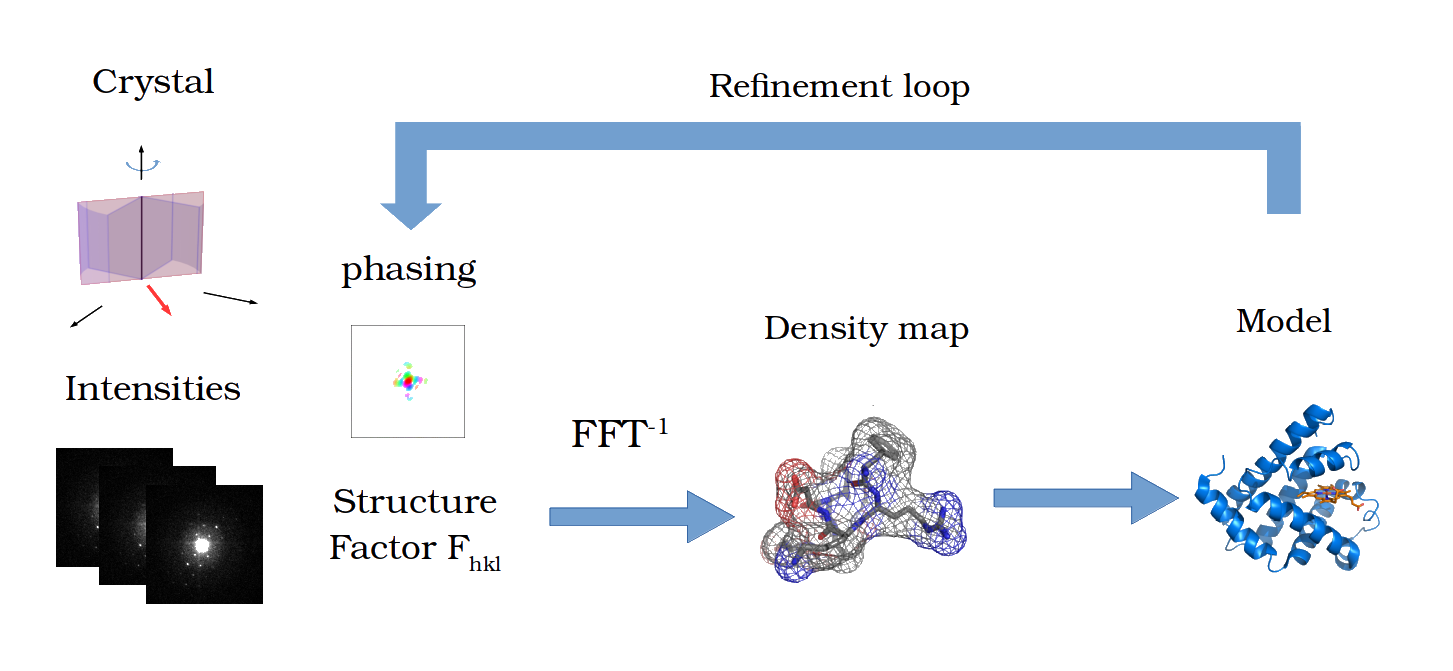
\includegraphics[width=\linewidth]{MX_t.png}
\end{center}
\vspace{-1em}
XD is based on the \emph{kinematic theory of diffraction} due to the
weak interaction between X-rays and the electron density.
Kinematic theory can not rigorously be applied to ED.


\mbox{\hspace{0.3\linewidth}\rule{0.4\linewidth}{1pt}\hspace{0.3\linewidth}}\\
\vspace{-1em}
\begin{center}\textbf{Schr$\ddot{o}$dinger fast electron wave equation}\end{center}

In ED, the structure factor is related to the electrostatic potential
through :
\begin{empheq}[box=\widecolourbox]{equation*}
	\frac{\dP\Psi(x,y,z)}{\dP_z} =
		\Big\{ \frac{i\lambda}{4\pi}\grad^2_{xy} + i\sigma V(x,y,z)\Big\}
\end{empheq}


\mbox{\hspace{0.3\linewidth}\rule{0.4\linewidth}{1pt}\hspace{0.3\linewidth}}\\
\vspace{-1em}
\begin{center}\textbf{Particle oriented picture}\end{center}
\begin{center}
	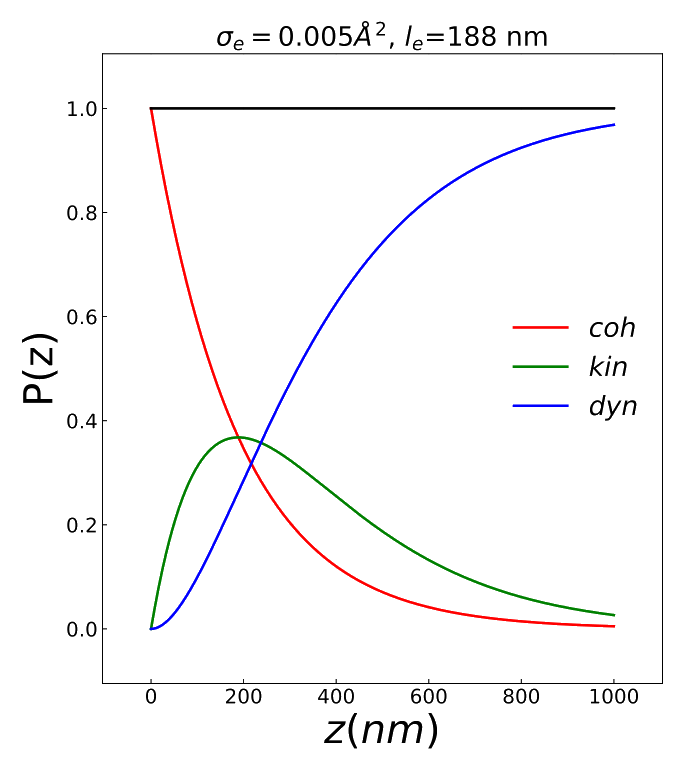
\includegraphics[width=0.5\linewidth]{fig/nearBragg/Pcoh_kin_dyn2.png}
\end{center}
% \vspace{-1em}
200keV electrons have typical elastic mean free path of 200nm in organic atoms.
This results in an appreciable probability of multiple scattering in nanocrystals.
\vspace{1.15em}
}





%%%%%%%%%%%%%%%%%%%%%%%%%%%%%%%%%%%%%%%%%%%%%%%%%%%%%%%%%%%%%%%%%%%%%%
%%%%%%%%%%%%%%%%%%%%%%%%%%%%%%%%%%%%%%%%%%%%%%%%%%%%%%%%%%%%%%%%%%%%%%
%%% Methods
%%%%%%%%%%%%%%%%%%%%%%%%%%%%%%%%%%%%%%%%%%%%%%%%%%%%%%%%%%%%%%%%%%%%%%
%%%%%%%%%%%%%%%%%%%%%%%%%%%%%%%%%%%%%%%%%%%%%%%%%%%%%%%%%%%%%%%%%%%%%%
\headerbox{Multislice(MS) method ~\cite{Kirkland2019}}{name=multi,column=1,span=1}{

	The sample is \highlight{sliced in real space} into regular slices $\Delta z$ and the solution is propagated from slice to slice through:
	$$\Psi(z+\Delta z) = \cc F^{-1}\Bigg\{p(k_x,k_y) \cc F\Big(e^{i\sigma\nu_{\Delta_z}(z)} \Psi(z)\Big) \Bigg\}$$

	% \begin{empheq}[box=\widecolourbox]{equation*}
	% 	\Psi(z+\Delta z) = \cc F^{-1}\Bigg\{p(k_x,k_y) \cc F\Big(e^{i\sigma\nu_{\Delta_z}(z)} \Psi(z)\Big) \Bigg\}
	% \end{empheq}

	where the Fresnel propagator $p(k_x,k_y)=e^{-i\pi\lambda\Delta z(k_x^2+k_y^2)}$,
	$\nu_{\Delta_z}=\int_z^{z+\Delta z}V(x,y,z^{'})dz^{'}$ is the projected potential.
	\vspace{0.65em}\\
	\begin{tabular}{@{}c@{ }c@{ }c@{ }}
		\hspace{1em}
		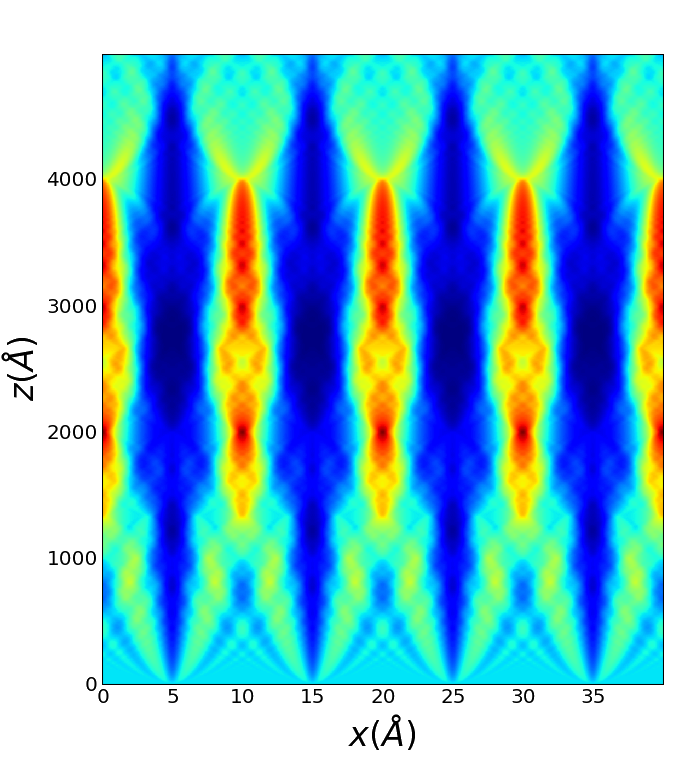
\includegraphics[width=0.45\linewidth]{fig/multislice/multi2D/multi2D_Q.png}&
		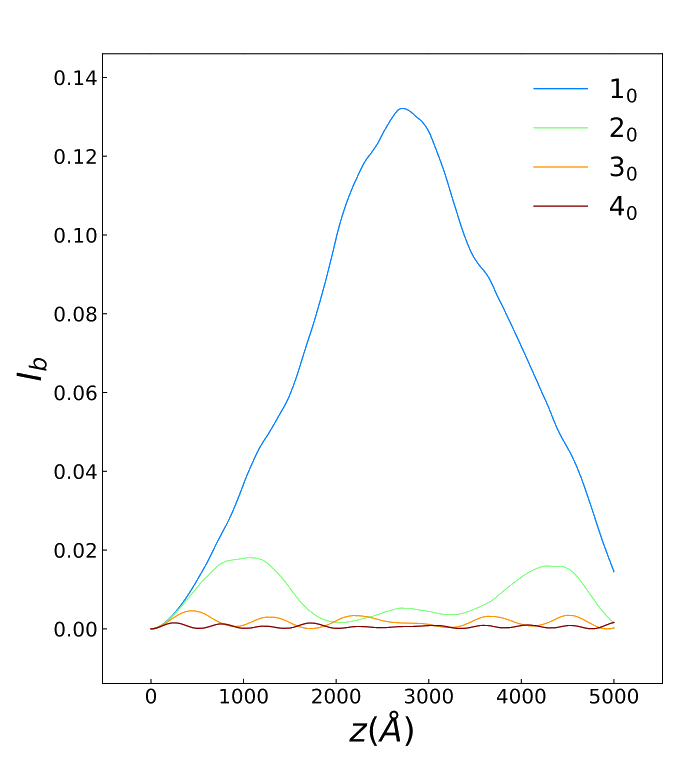
\includegraphics[width=0.45\linewidth]{fig/multislice/multi2D/multi2D_Z.png}\\
        \smaller a) Typical $\Psi(x,z)$ & \smaller b) Strong beams intensities
  \end{tabular}

	\vspace{0.5em}
	\begin{itemize}\compresslist
	 \item The Discrete Fourier Transform $\cc F$ provides \highlight{fast and efficient $N\log N$ time complexity}.% with beam number $N$.
	 \item \negCol{Padding and large transverse super cells} necessary for non zone-axis orientations.
	 \item Possiblity to model \highlight{solvent,inelastic scattering, disorder, partial coherency...}.
	\end{itemize}

Padded simulation for a IRELOH  : % found in continuous rotation experiment:

	\begin{tabular}{@{}c@{ }c@{ }c@{ }}
		\hspace{1em}
		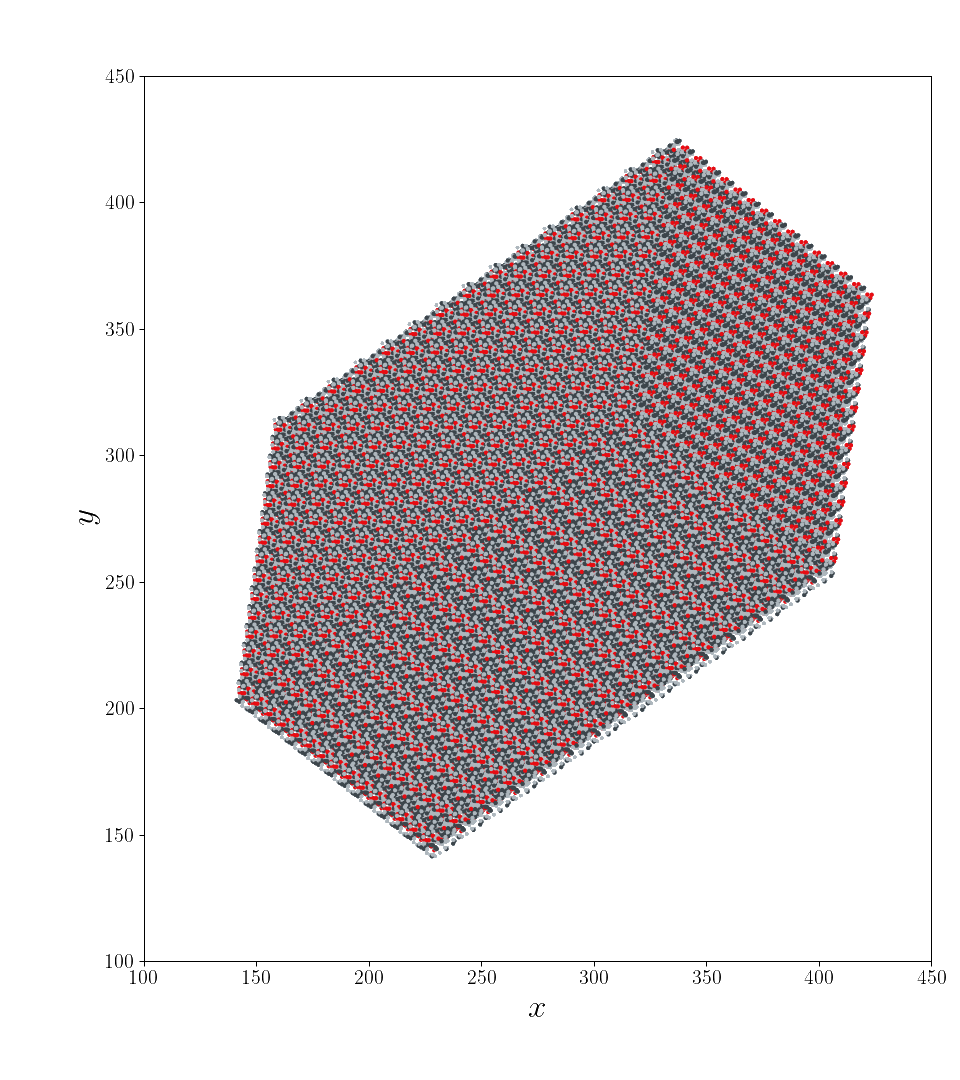
\includegraphics[width=0.45\linewidth]{fig/multislice/ireloh/multislice_ireloh_xy.png}&
		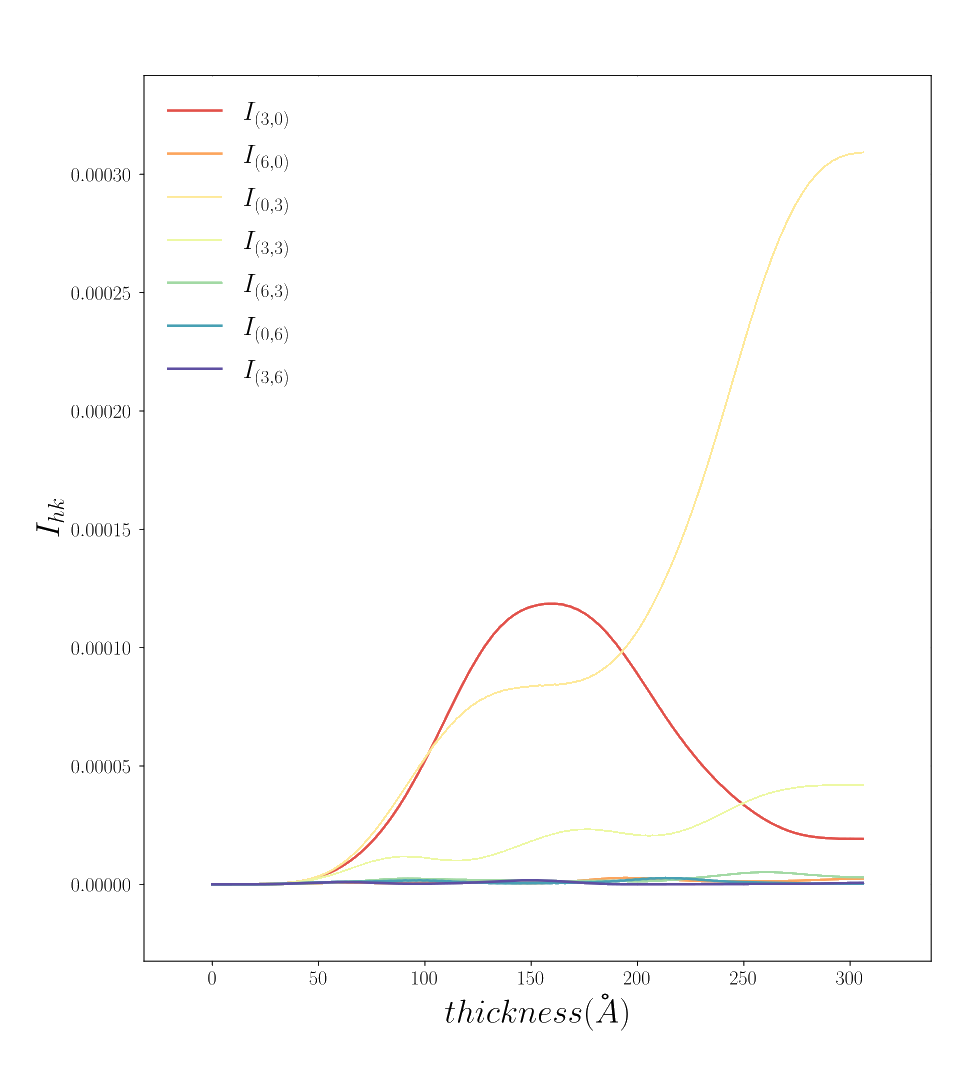
\includegraphics[width=0.45\linewidth]{fig/multislice/ireloh/484_B.png}\\
      \smaller a) real space setup & \smaller b) strong beams intensities
  \end{tabular}
\vspace{0.25em}
}


%%% Blochwave
%%%%%%%%%%%%%%%%%%%%%%%%%%%%%%%%%%%%%%%%%%%%%%%%%%%%%%%%%%%%%%%%%%%%%%
\headerbox{Blochwave(BW) approach~\cite{Zuo1995}}{name=bloch,column=2,span=1}{
	% The sample is assumed to be an infinite periodic crystal.
	The wave function is \highlight{solved in reciprocal space} by finding the
	eigen values $\gamma_j$ and eigen vectors $C_{j,\bb G}$:
	$$S_{\bb G}C_{j,\bb G} + \sum_{\bb G^{'}}\frac{U_{\bb G-\bb G^{'}}}{2k_0} C_{j,\bb G^{'}} = \gamma_jC_{j,\bb G}$$

	% \begin{empheq}[box=\widecolourbox]{equation*}
	% 	S_{\bb G}C_{j,\bb G} + \sum_{\bb G^{'}}\frac{U_{\bb G-\bb G^{'}}}{2k_0} C_{j,\bb G^{'}} = \gamma_jC_{j,\bb G}
	% \end{empheq}

	The diffracted intensities of the strong beams $\bb G$ (small excitation
	error $S_{\bb G}$) are computed for any thickness sample $H$ with
	$I_{\bb G}=|\bb C\bb e^{2i\pi\boldsymbol{\gamma_j}H}\bb C^{-1}|^2$.

	\begin{tabular}{@{}c@{ }c@{ }c@{ }}
		\hspace{1em}
		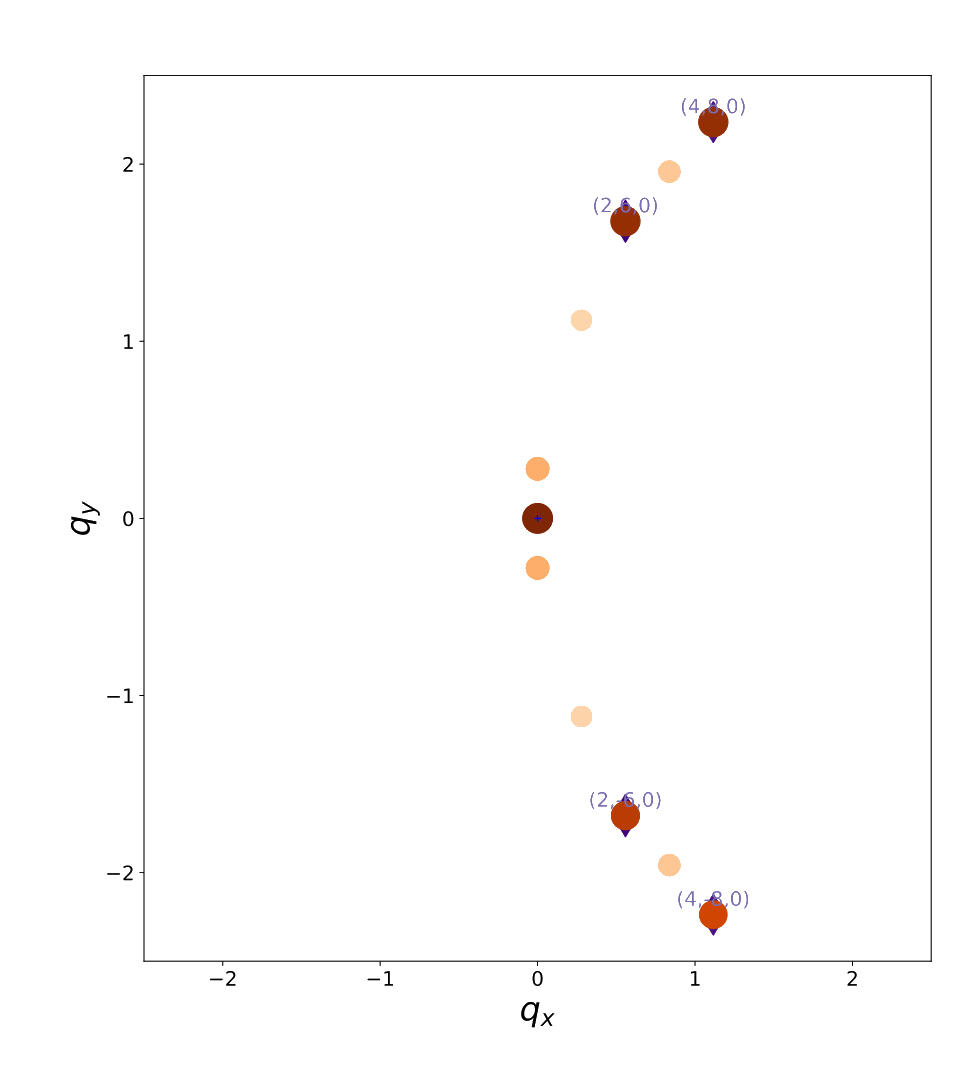
\includegraphics[width=0.45\linewidth]{fig/bloch/bloch_Sw.png}&
		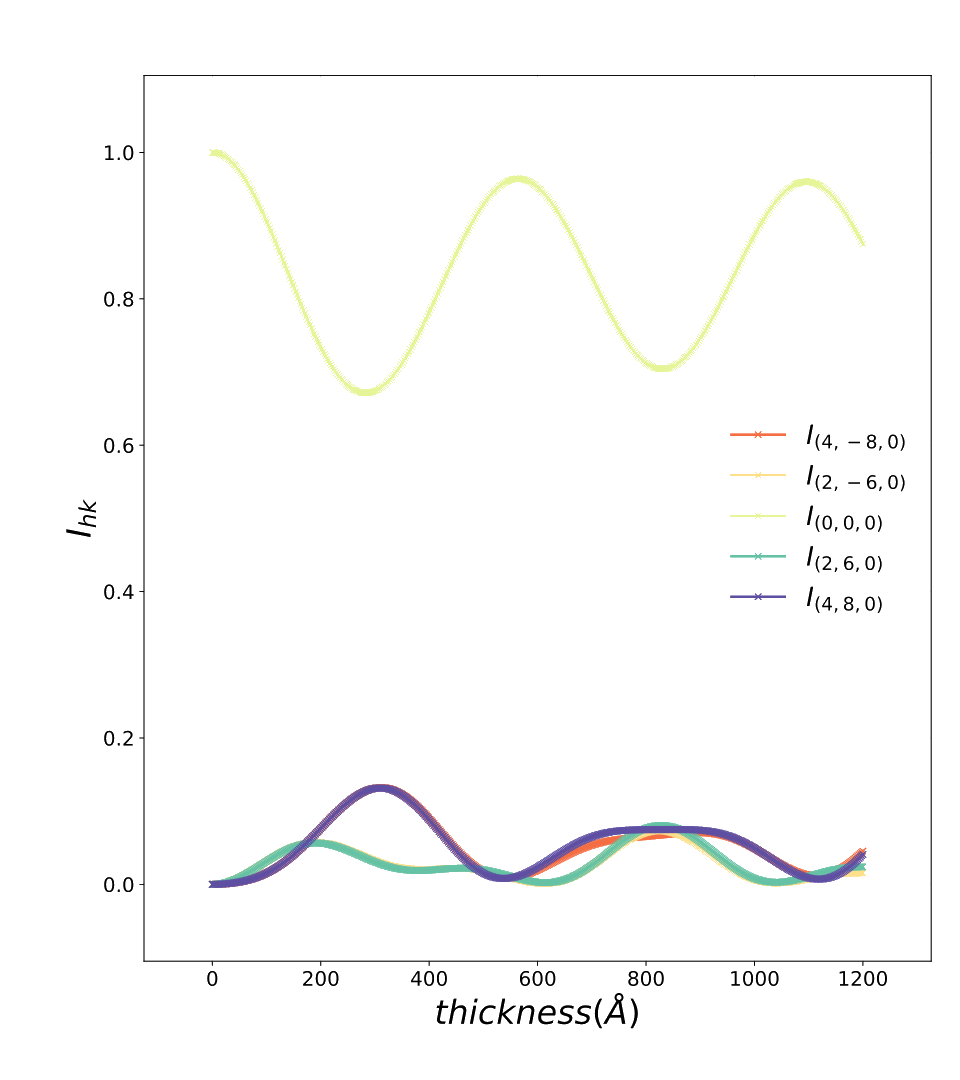
\includegraphics[width=0.45\linewidth]{fig/bloch/bloch_Iz.png}\\
      \smaller a) $S_{\bb G}$ and potential $U_{\bb G}$ & \smaller b) Strong beams intensities $I_{\bb G}$
  \end{tabular}

	\vspace{0.5em}
	\begin{itemize}\compresslist
	 \item Diagonalization \negCol{time complexity scales as $N^3$} but \highlight{only strongest beams need be included}.
	 \item \highlight{Random orientations of any lattice} can be simulated.
	 \item Inelastic scattering can be modelled but \negCol{not solvent scattering, disorder and defects}.
	\end{itemize}


 Rocking curves for diamond in different configurations :

	\begin{tabular}{@{}c@{ }c@{ }c@{ }}
		\hspace{1em}
		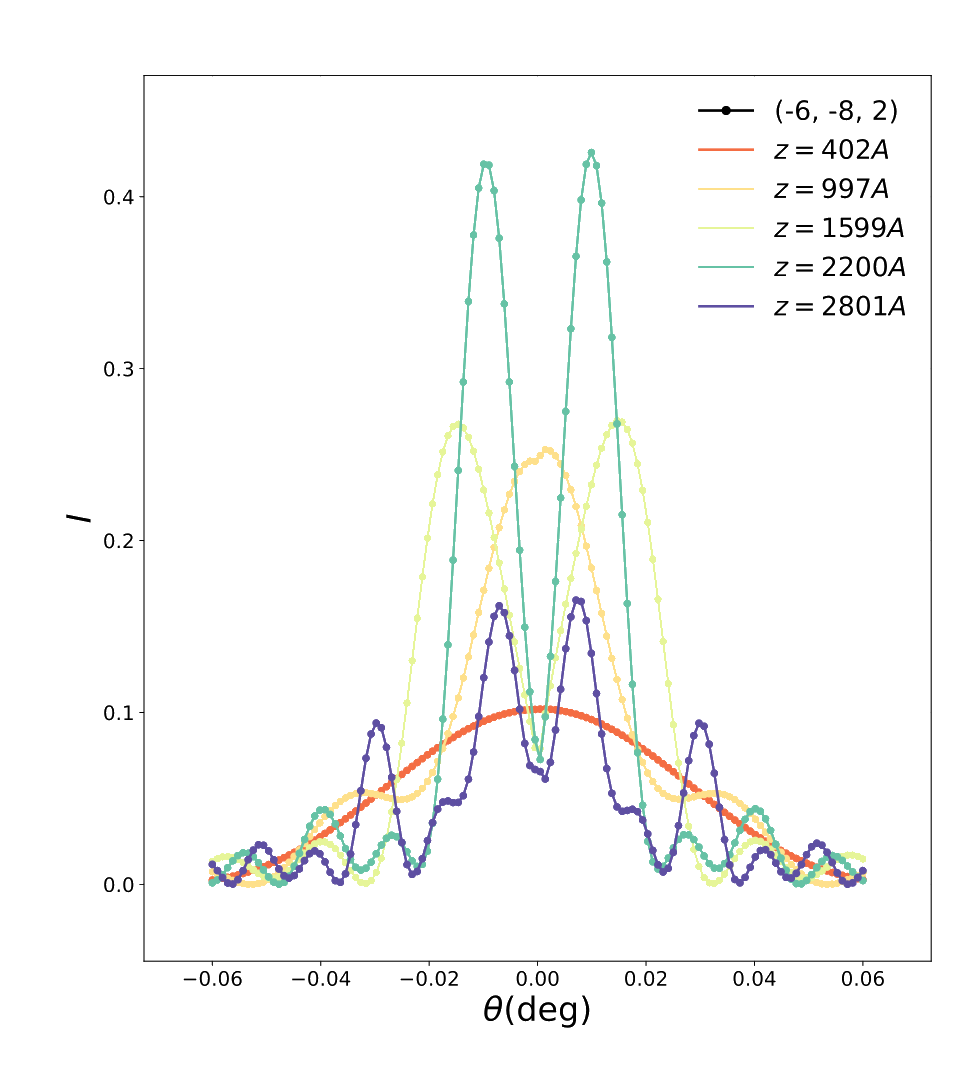
\includegraphics[width=0.45\linewidth]{fig/bloch/diamond_rock2.png}&
		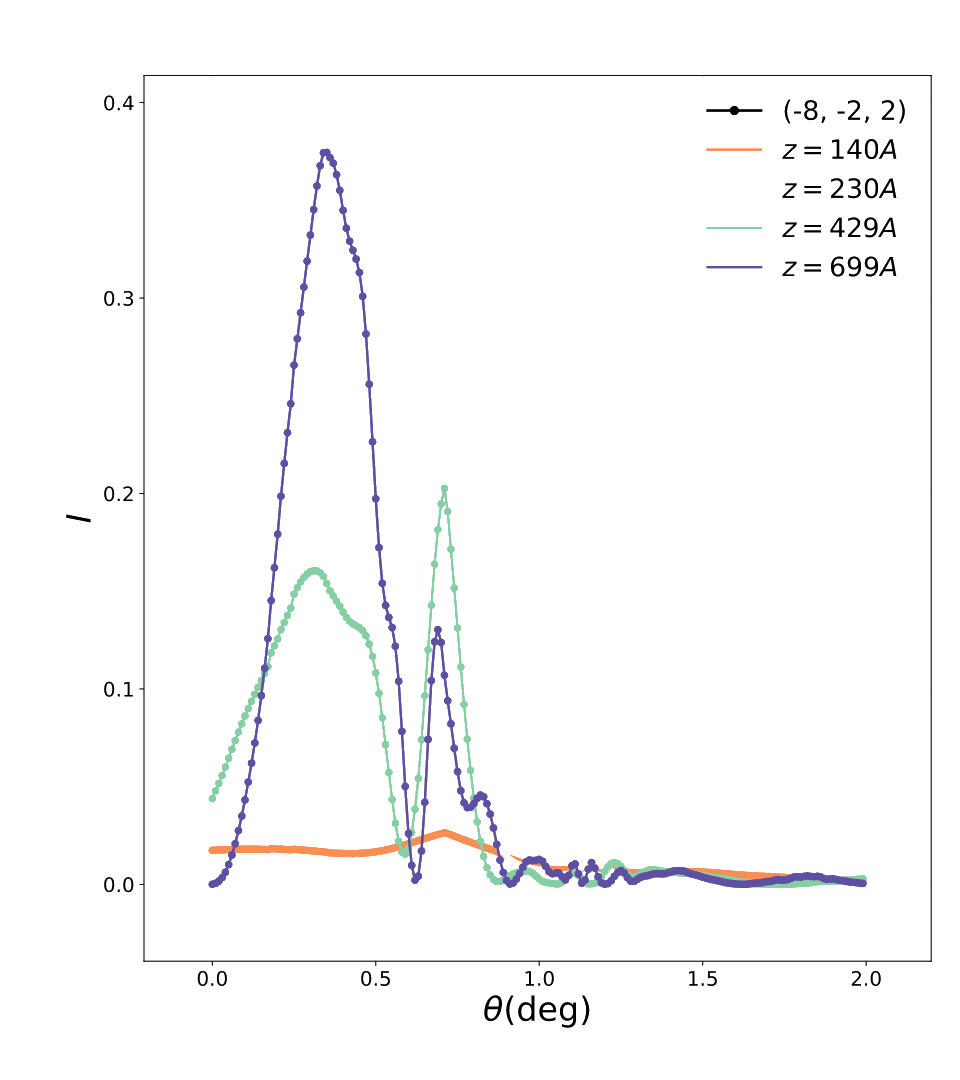
\includegraphics[width=0.45\linewidth]{fig/bloch/diamond_rock1.png}\\
      \smaller a) 3 beam setup & \smaller b) arbitrary orientation
  \end{tabular}
}



%%%%%%%%%%%%%%%%%%%%%%%%%%%%%%%%%%%%%%%%%%%%%%%%%%%%%%%%%%%%%%%%%%%%%%
%%%%%%%%%%%%%%%%%%%%%%%%%%%%%%%%%%%%%%%%%%%%%%%%%%%%%%%%%%%%%%%%%%%%%%
%%% Results
%%%%%%%%%%%%%%%%%%%%%%%%%%%%%%%%%%%%%%%%%%%%%%%%%%%%%%%%%%%%%%%%%%%%%%
%%%%%%%%%%%%%%%%%%%%%%%%%%%%%%%%%%%%%%%%%%%%%%%%%%%%%%%%%%%%%%%%%%%%%%
\headerbox{Application to $\alpha$-glycine}{name=glycine,column=1,span=2,below=multi}{

\begin{multicols}{2}

	Experimental continuous rotation electron diffraction dataset of $\alpha$-glycine
	% \vspace{0.5em}

	\begin{tabular}{@{}c@{ }c@{ }c@{ }c@{ }c@{ }c@{ }c@{ }c@{ }c@{ }}
		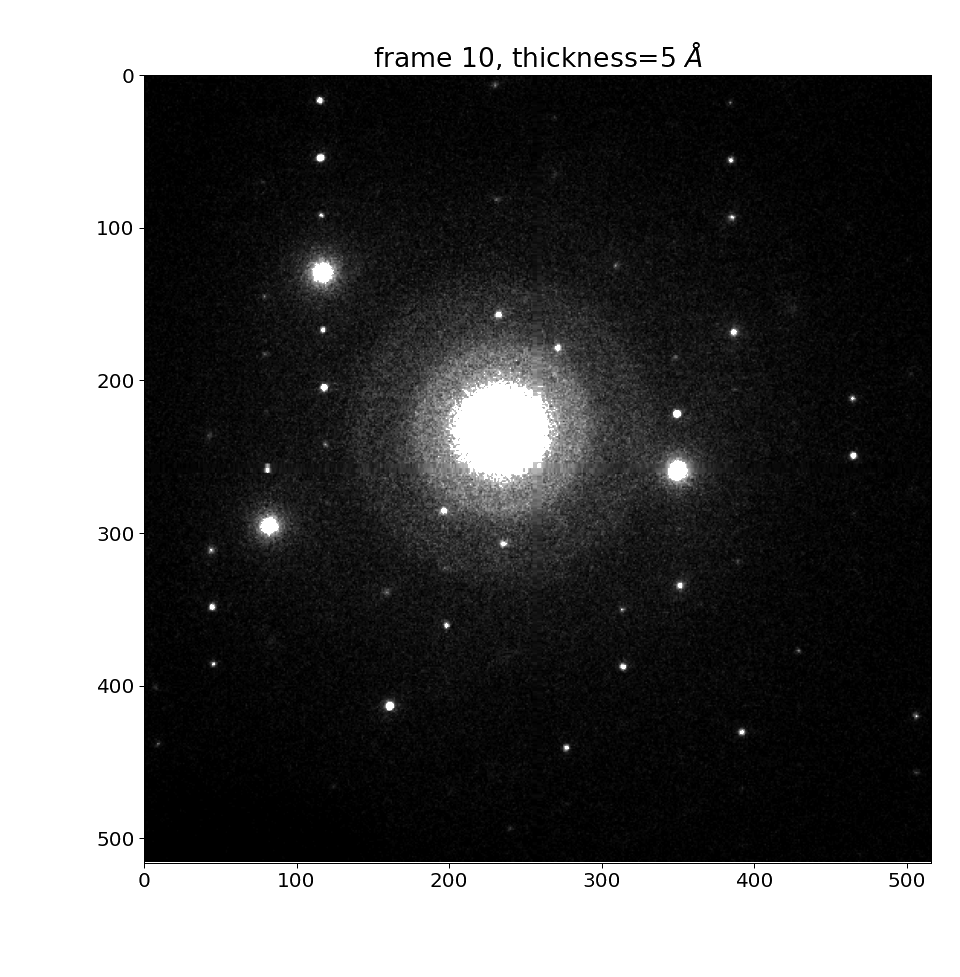
\includegraphics[width=0.33\linewidth]{fig/glycine/_009.png}&
		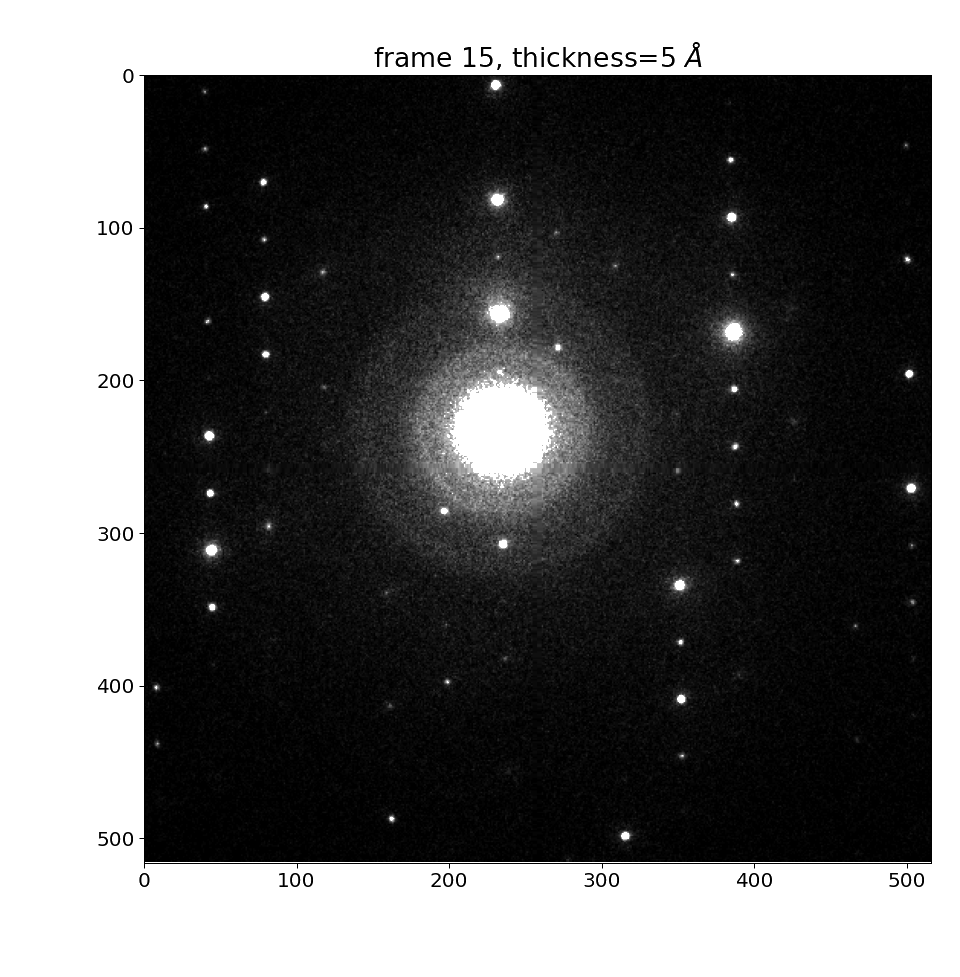
\includegraphics[width=0.33\linewidth]{fig/glycine/_014.png}&
		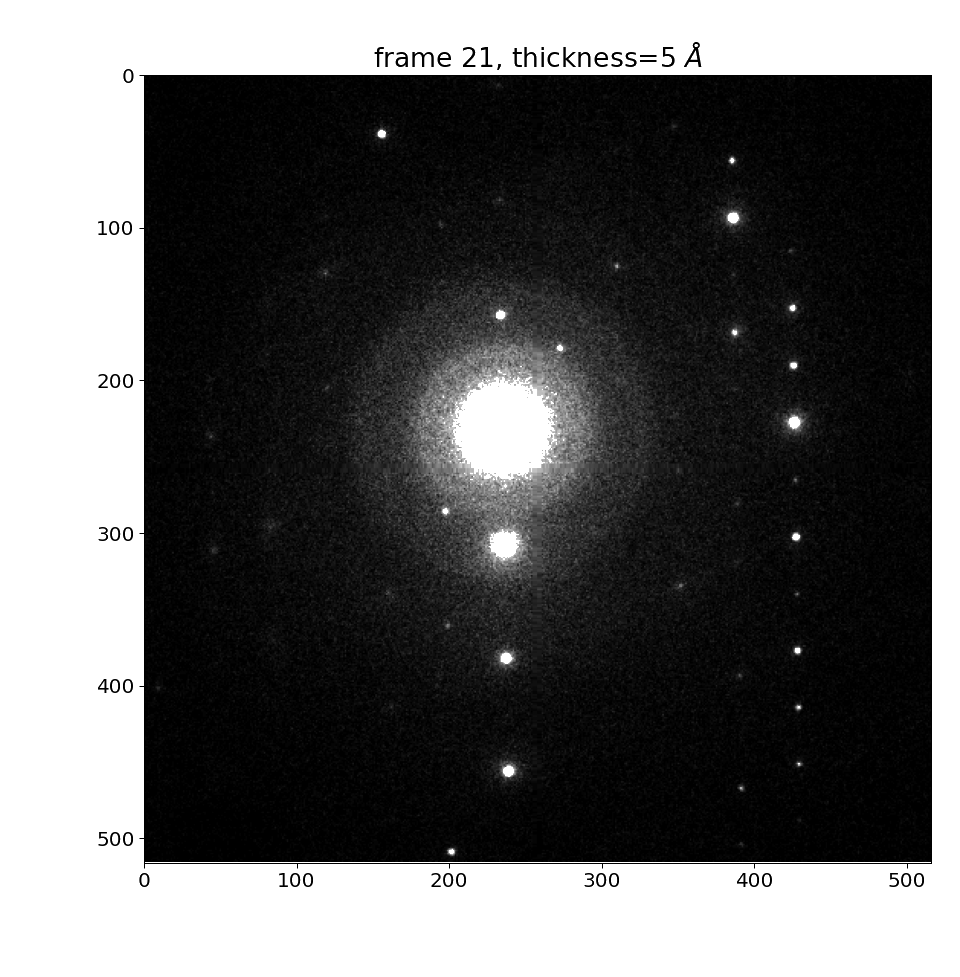
\includegraphics[width=0.33\linewidth]{fig/glycine/_020.png}\\
			 a) frame 10 & \smaller b) frame 15 & \smaller c) frame 21
	\end{tabular}

	\vspace{1em}
	Simulated frames using multislice. Padding was used to simulate
	the experimental orientations as retrieved by data processing
	software PETS2(\url{http://pets.fzu.cz/})

	\begin{tabular}{@{}c@{ }c@{ }c@{ }c@{ }c@{ }c@{ }c@{ }c@{ }c@{ }}
		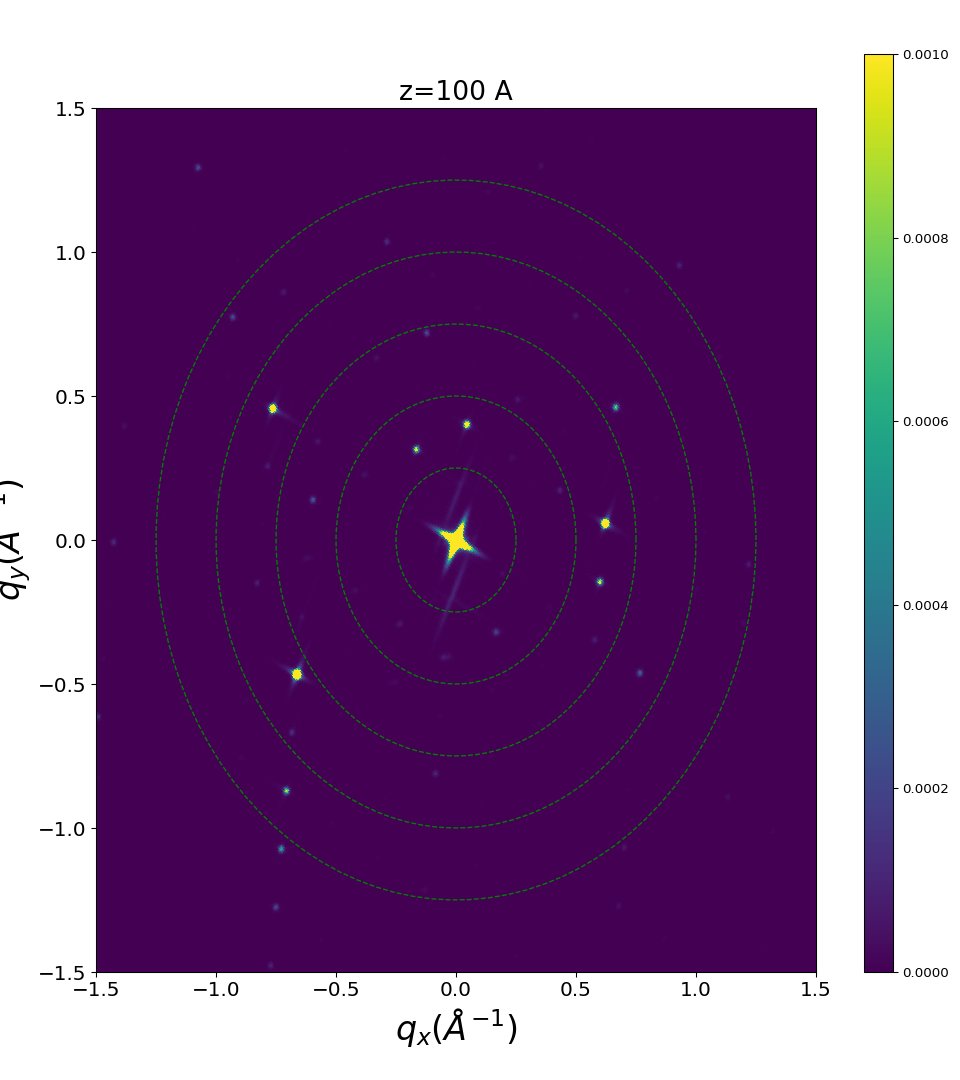
\includegraphics[width=0.33\linewidth]{fig/multislice/glycine/glycine_test10.png}&
		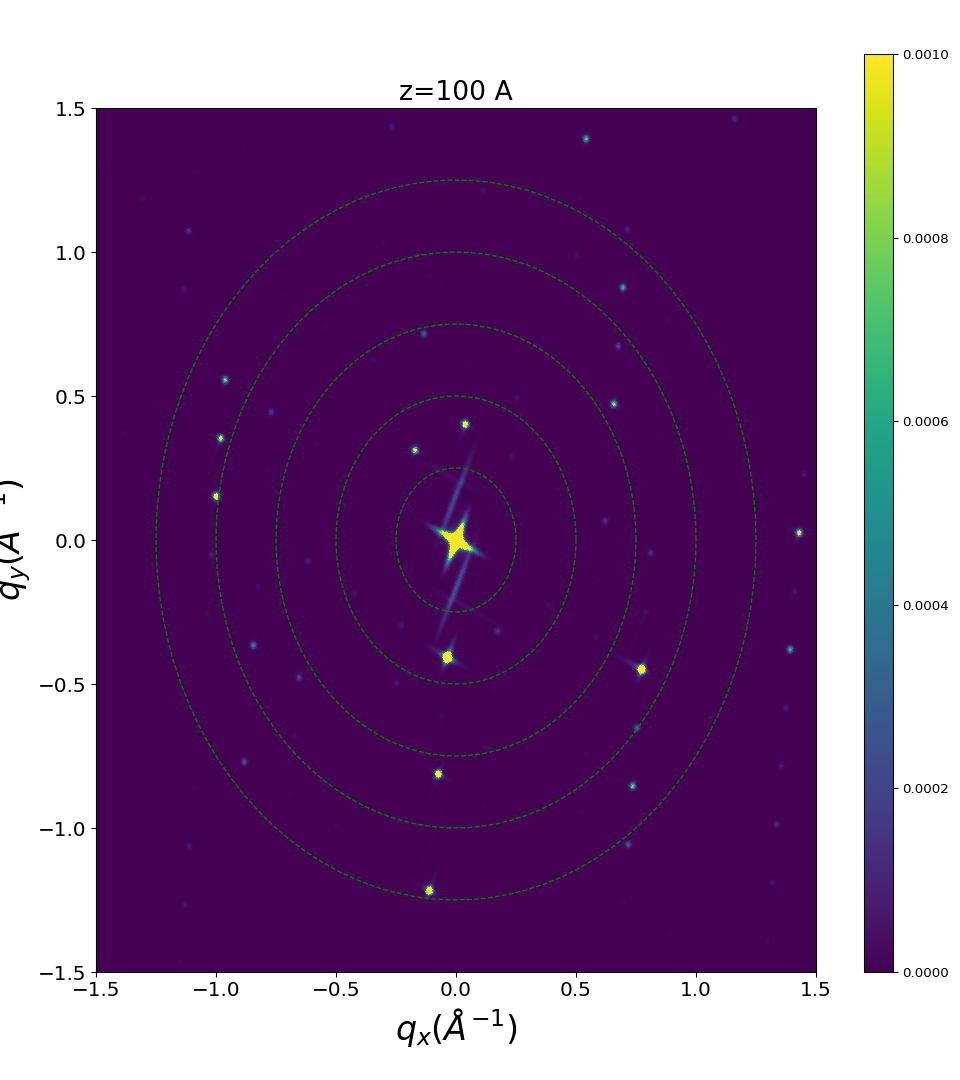
\includegraphics[width=0.33\linewidth]{fig/multislice/glycine/glycine_test15.png}&
		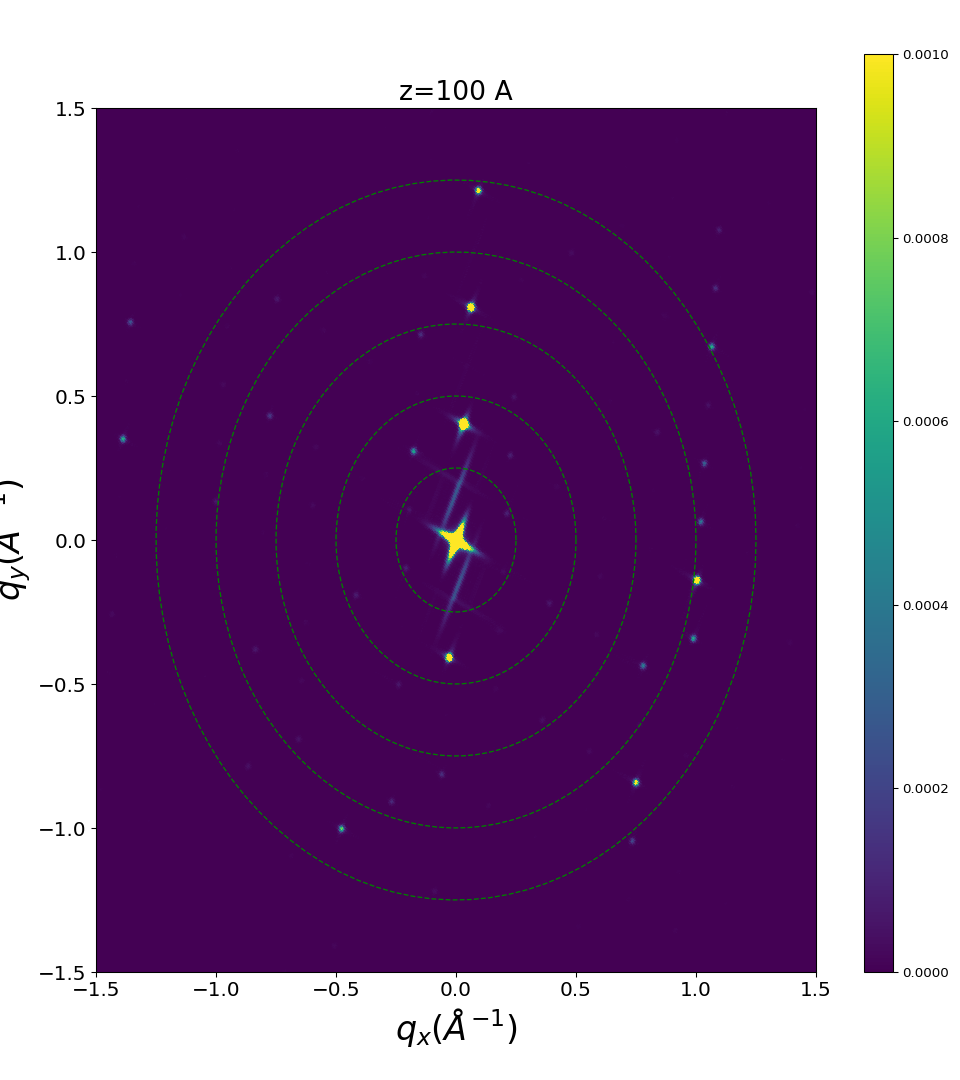
\includegraphics[width=0.33\linewidth]{fig/multislice/glycine/glycine_test21.png}\\
			 a) frame 10 & \smaller b) frame 15 & \smaller c) frame 21
	\end{tabular}

\vspace{1em}
The main reflections are correctly predicted, although the patterns need to be rotated
in the plane of the figure to get an exact match. The reflection broadening is related to
finite size effects and window function of the padded domain.

Excitation errors ($-\log_{10}(S_{\bb G})$) of main beams over frames [1-30] and
simulated rocking curve of main reflection (0,0,2):

\begin{tabular}{@{}c@{ }c@{ }c@{ }c@{ }c@{ }}
	\hspace{1em}
	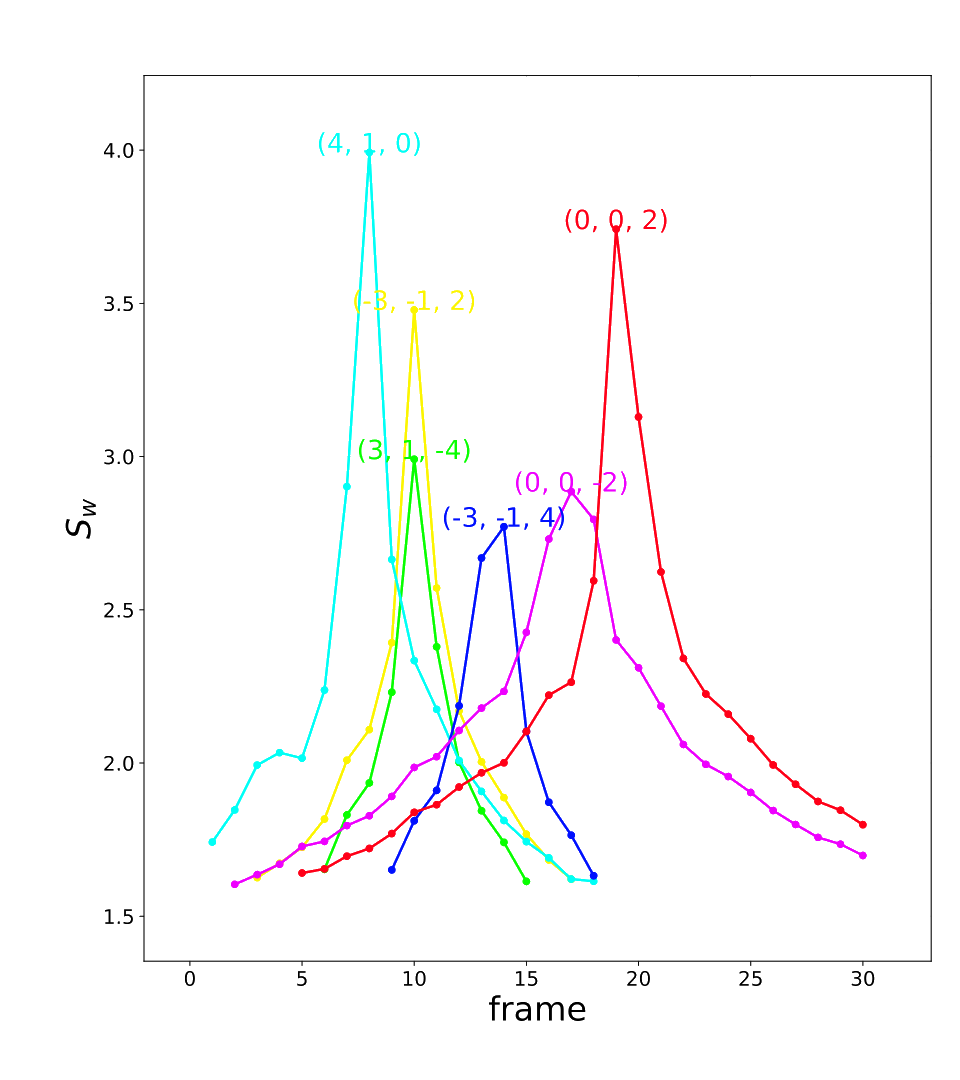
\includegraphics[width=0.45\linewidth]{fig/glycine/glycine_theta_Sw.png}&
	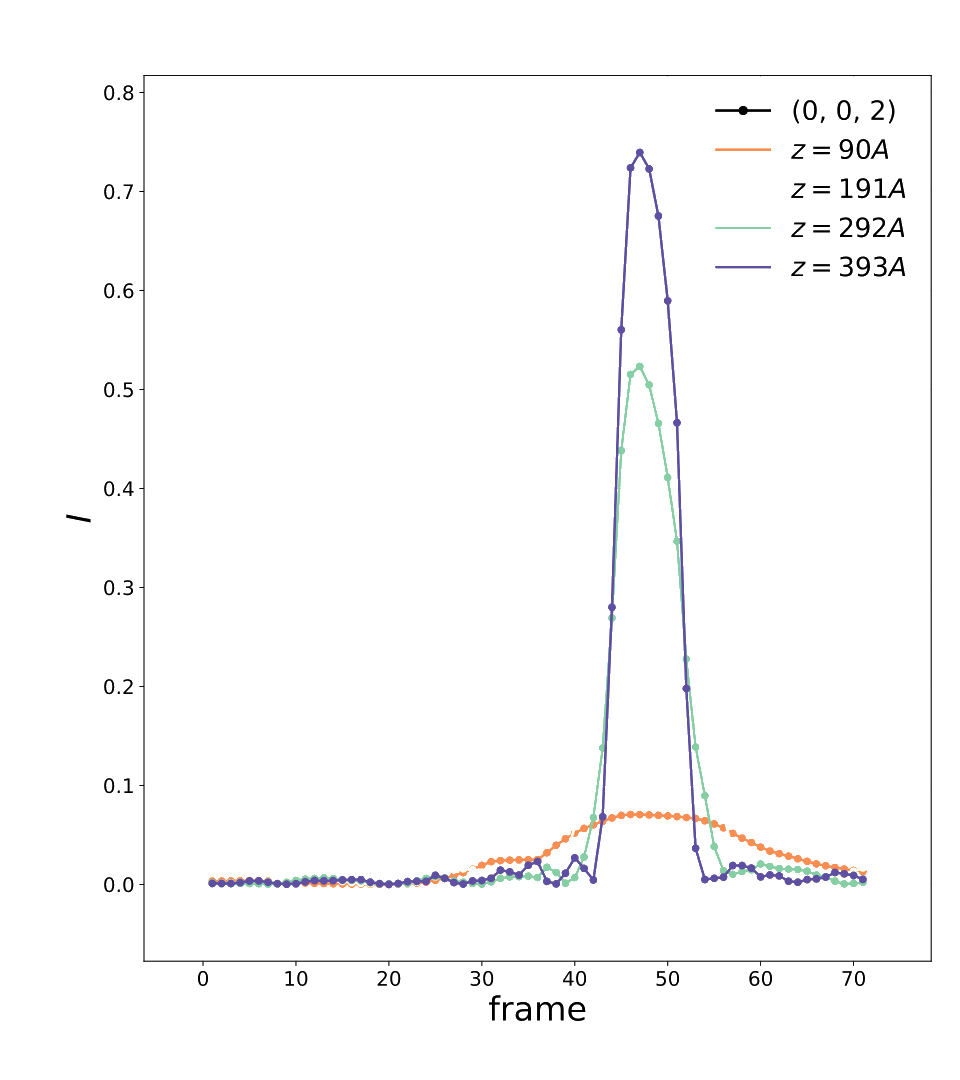
\includegraphics[width=0.45\linewidth]{fig/glycine/glycine_ref_beams5.png}\\
		 \smaller a) Excitation error & \smaller b) Rocking curve for (0,0,2)
\end{tabular}

\vspace{1em}
Experimental intensities :

\begin{tabular}{@{}c@{ }c@{ }c@{ }c@{ }c@{ }}
	\hspace{1em}
	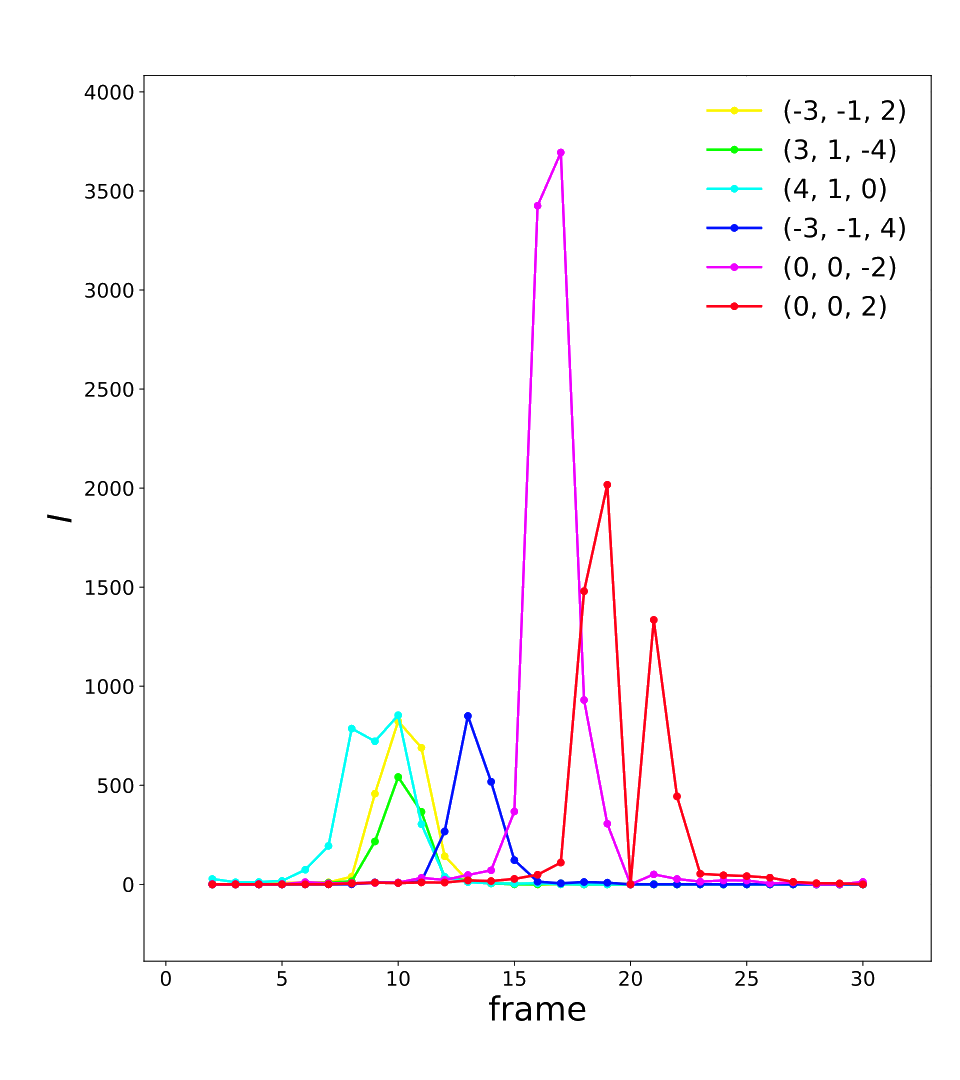
\includegraphics[width=0.45\linewidth]{fig/glycine/glycine_Iframe.png}&
	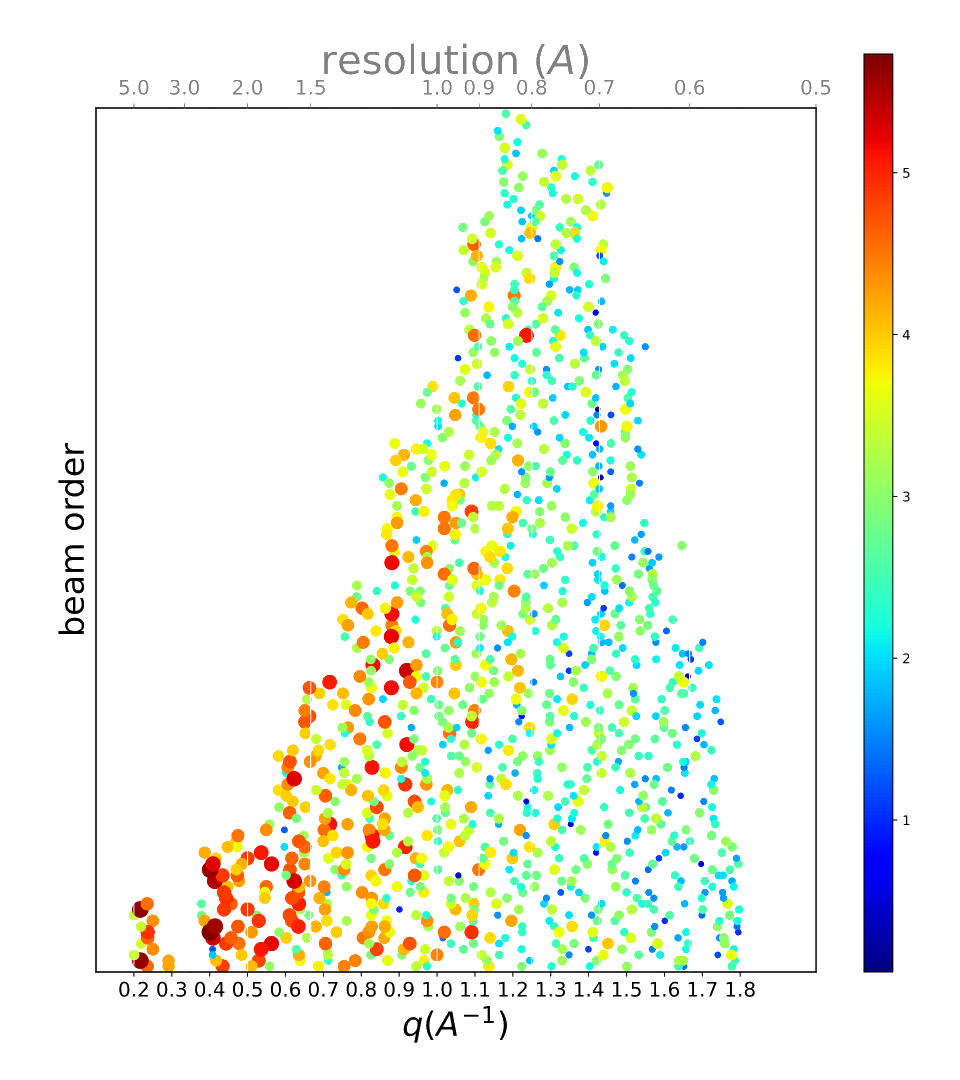
\includegraphics[width=0.45\linewidth]{fig/glycine/glycine_Ihkl.png}\\
		\smaller a) Experimental intensities & \smaller b) Distribution with resolution
\end{tabular}

% \vspace{1em}
\end{multicols}

\vspace{0.2em}
}

%%%%%%%%%%%%%%%%%%%%%%%%%%%%%%%%%%%%%%%%%%%%%%%%%%%%%%%%%%%%%%%%%%%%%%
%%%%%%%%%%%%%%%%%%%%%%%%%%%%%%%%%%%%%%%%%%%%%%%%%%%%%%%%%%%%%%%%%%%%%%
%%%%%%%%%%%%%%%%%%%%%%%%%%%%%%%%%%%%%%%%%%%%%%%%%%%%%%%%%%%%%%%%%%%%%%
%%% ref, ack
%%%%%%%%%%%%%%%%%%%%%%%%%%%%%%%%%%%%%%%%%%%%%%%%%%%%%%%%%%%%%%%%%%%%%%
%%%%%%%%%%%%%%%%%%%%%%%%%%%%%%%%%%%%%%%%%%%%%%%%%%%%%%%%%%%%%%%%%%%%%%
%%%%%%%%%%%%%%%%%%%%%%%%%%%%%%%%%%%%%%%%%%%%%%%%%%%%%%%%%%%%%%%%%%%%%%
\headerbox{References}{name=references,column=0,span=2,above=bottom}{
\smaller																  % Make the whole text smaller
\vspace{-0.4em} 												  % Save some space at the beginning
% \bibliographystyle{alpha}	 								% Use plain style
\renewcommand{\section}[2]{\vskip 0.05em}	% Omit "References" title
\input{refs.bbl}
}
\headerbox{Acknowledgements}{name=acknowledgements,span=1,column=2, above=bottom}{
% \smaller						% Make the whole text smaller
% \vspace{0.1em}			% Save some space at the beginning
This research was supported by BBSRC grant WP4. The supports are gratefully acknowledged.
}
\end{poster}
\end{document}
